% ********** Chapter 1 **********
\section{Design}
\label{sec:chap1:design}

Eine JSR 223 Implementation f"ur PHP besteht gezwungenermassen aus zwei Teilen: einem Java-Teil, welcher im Wesentlichen
die ScriptEngineFactory enth"alt, komplett in Java ohne die Verwendung von nativen (JNI-) Aufrufen implementiert ist und
s"amtliche Funktionalit"at des Auffindungsmechanismus abdeckt, sowie einem nativen Teil, welcher aus 
einem C- oder C++ - Programm, das die n"otigen Aufrufe an PHP vornimmt besteht.
Die eigentliche ScriptEngine verbindet diese beiden Teile indem sie aus Java heraus dieses, in nativen Code "ubersetzte, 
Programm mittels JNI anspricht.
Um allerdings JSR 223 "uberhaupt nutzen zu k"onnen m"ussen die Klassen aus javax.script, vor allem der ScriptEngineManager, 
im Java-Classpath liegen. Hierzu kann entweder eine Java-Runtime der Version 6, oder aber eine eigene Implementation dieser
Klassen genutzt werden. Wichtige Use-Cases f"ur diesen Teil des Projektes sind:
\begin{enumerate}
\item Test, ob die PHP-ScriptEngine verf"ugbar ist. Durch einfache Ausgabe auf der Konsole soll schnell ermittelbar sein, welche
    ScriptEngines geladen und einsatzbereit sind. Dies dient haupts"chlich der "Uberpr"ufung, ob die aktuelle Java-Umgebung
    richtig konfiguriert ist.
\item Test, ob die PHP-ScriptEngine funktioniert. Es soll ein einfaches PHP-Skript ausgef"uhrt werden, um dem Anwender
    die korrekte Funktionsweise der ScriptEngine vorzuf"uhren und zu pr"ufen ob die nativen Teile der Implementation
    ordnungsgem"a\ss funktionieren.
\item Ausf"uhren beliebiger PHP-Skripte. Es soll dem Anwender m"oglich sein, ohne selbst Java-Quelltext zu schreiben, beliebige
    PHP-Skripte auszuf"uhren.
\item "Ubersetzen eines beliebigen Skriptes. Gem"a\ss des in \emph{javax.script} vorhandenen Interfaces \emph{Compilable} soll 
    ein beliebiges Skript "ubersetzt und mehrfach ausgef"uhrt werden k"onnen.
\item Aufrufen von Methoden in "ubersetzten Skripten. Das zu entwickelnde Softwaresystem soll das Aufrufen von Funktionen und
    Methoden in "ubersetzten Skripten erlauben. Hierzu soll das Interface \emph{javax.script.Invocable} unterst"utzt werden.
\item "Ubergabe von Daten mittels des Kontextes. Der Anwender soll Daten mittels des Engine-Kontextes "ubergeben und in PHP
    weiterverwenden k"onnen. Genauso soll es m"oglich sein Daten aus PHP heraus an die JVM zur"uckzu"ubergeben.
\item Setzen von php.ini Parametern. Dem Anwender soll die M"oglichkeit geboten werden eine alternative php.ini Datei zu verwenden,
    um das Laufzeitverhalten von PHP wie gewohnt zu beeinflussen.
\end{enumerate}
Die im folgenden beschriebene JSR 223 Implementation tr"agt den Namen "'Turpitude"'.

\subsection{Java}
\label{sec:chap1:design:java}

Um f"ur den ScriptEngineManager auffindbar zu sein muss eine JSR 223 Implementation sich gem"ass der \emph{Jar File Specification} \cite{JARSPEC} 
als sogenannter \emph{Service Provider} registrieren. Hierzu muss sich im Verzeichnis \emph{META-INF/services} des .jars eine Datei
mit dem Namen der Service-Klasse (in diesem Fall \emph{javax.script.ScriptEngineFactory}) befinden, in welcher verf"ugbare 
ScriptEngineFactories zeilenweise aufgelistet werden.

Alle Klassen der Implementation befinden sich im Package \emph{net.xp\_framework.turpitude}. 
Die ScriptEngineFactory-Implementation hei\ss t \emph{PHPScriptEngineFactory} und implementiert direkt das Interface 
\emph{ScriptEngineFactory} aus \emph{javax.script}. Im Gegensatz dazu implementiert die Klasse \emph{PHPScriptEngine} nicht
direkt das Interface \emph{ScriptEngine}, sondern erbt von der abstrakten Klasse \emph{AbstractScriptEngine}, welche f"ur
viele Varianten der \emph{eval()}-Methode schon eine Realisierung, sowie mit der Klasse \emph{SimpleScriptContext} schon einen 
\emph{ScriptContext} mitbringt. Um den "ubergebenen Scriptcode tats"achlich auszu"fuhren muss dieser an den mittels der Java-Methode
\emph{System.loadLibary()} geladenen nativen Teil der Implementation weitergegeben werden. Die Kommunikation mit diesem
nativen Teil findet mittels JNI-Methoden statt.
Weiterhin implementiert die PHPScriptEngine die beiden in \emph{javax.script} enthaltenen Interfaces \emph{Compilable} und
\emph{Invocable}, deren Funktionalit"at zur Erff"ullung einiger der Use-Cases ben"otigt wird. F"ur die Methoden aus
Compilable wird noch eine weitere Klasse - \emph{PHPCompiledScript} - erstellt, welche direkt von der abstrakten
Klasse \emph{javax.script.CompiledScript} erbt.

Die Kommunikation zwischen Java und PHP findet "uber zwei unterschiedliche Kan"ale statt:

Bei der R"uckgabe von Daten aus einem PHP-Skript werden diese einfach kopiert, wobei simple Datentypen (bool, long, double und string)
einfach in ihre Java-"Aquivalente (java.lang.Boolean, java.lang.Long, java.lang.Double und java.lang.String) umgesetzt werden.
Da alle Arrays in PHP assoziativer Natur sind werden sie als untypisierte java.util.HashMap, das heisst sowohl der Schl"ussel als auch der Wert
sind vom Typ java.lang.Object, zur"uckgegeben. Einzig f"ur PHP-Objekte wird eine gesonderte Java-Klasse ben"otigt: \emph{PHPObject} enth"alt neben
der Klassennamen auch alle Eigenschaften eines PHP-Objektes. Diese werden in einer HashMap gespeichert, mit dem Namen der Eigenschaft
als Schl"ussel.

Die Eingabe von Daten aus Java heraus in ein PHP-Skript geschieht - gem"a\ss der JSR223-Spezifikation - mittels des Kontextes der
ScriptEngine. Hierzu wird dieser - zusammen mit einigen Umgebungsvariablen und -Informationen - in eine globale Variable injiziert,
deren Name sich in der ScriptEngine setzen l"asst. Im Unterschied zu den oben beschriebenen R"uckgabewerten stellen die Kontext-Objekte
Referenzen dar, so wirken sich "Anderungen an diesen unmittelbar auf die entsprechenden Java-Objekte aus.


Die Abbildung \ref{fig:jsr223impl} zeigt die beteiligten Klassen und ihre Abh"anigkeiten untereinander,
zusammen mit einigen wichtigen Methoden und Attributen. 

\begin{figure}[h]
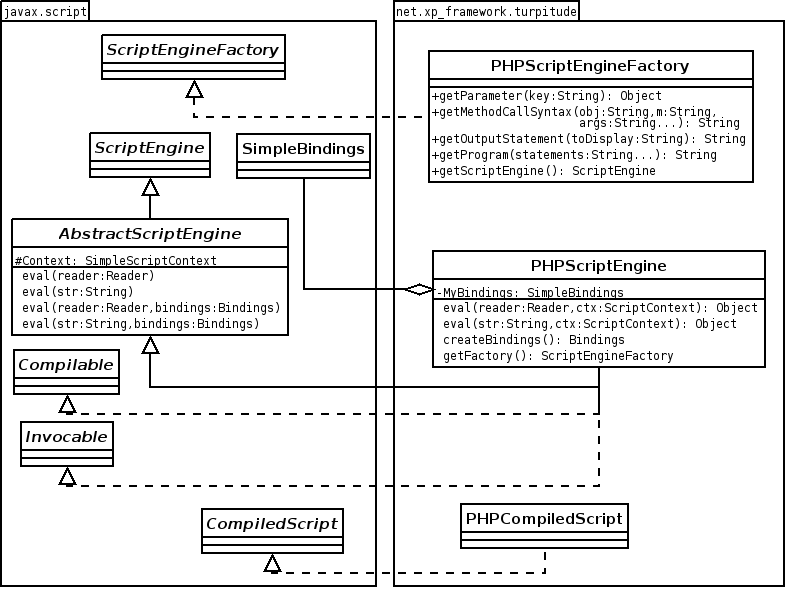
\includegraphics[width=\textwidth]{chap1/img/turpitude.png}
\caption{JSR 223 Implementation - Architektur}
\label{fig:jsr223impl}
\end{figure}

Der JSR 223 spezifiziert nur eine Exception (\emph{javax.script.ScriptException}) um alle m"oglichen Laufzeitfehler innerhalb einer 
Implementation abzudecken. Um dem Anwender trotzdem eine M"oglichkeit einer differenzierten Fehlerauswertung zu geben werden drei
zus"atzliche Exceptions eingef"uhrt: \emph{PHPScriptException}, \emph{PHPCompileException} und \emph{PHPEvalException} (siehe Abbildung
\ref{fig:jsr223exceptions}). Die PHPScriptException dient zum Einen als Oberklasse, zum anderen kann der Anwender durch sie erkennen, ob
das aufgetretene Problem implementationsspezifisch ist. Die beiden anderen neuen Exceptions werden genutzt um Fehler beim "Ubersetzen 
(PHPCompileException) oder beim Ausf"uhren (PHPEvalException) eines Skriptes voneinander abzugrenzen.

\begin{figure}[h]
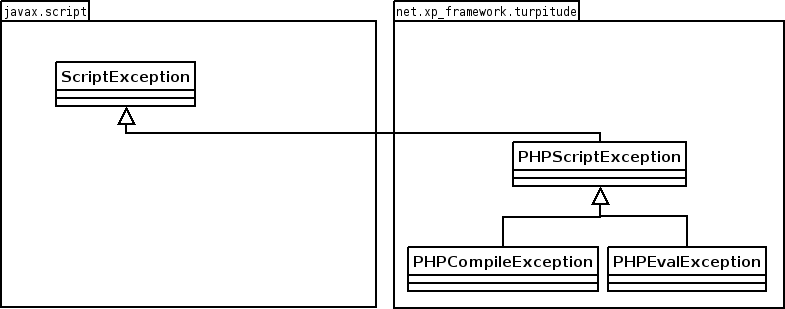
\includegraphics[width=\textwidth]{chap1/img/exceptions.png}
\caption{JSR 223 Implementation - Exceptions}
\label{fig:jsr223exceptions}
\end{figure}

\subsection{Native}
\label{sec:chap1:design:native}

Der native Teil der Implementation teilt sich wiederum auf in JNI-Methoden, f"ur welche die Headerdateien automatisch aus
der Java-Klasse der PHPScriptEngine generiert werden k"onnen, und in die Implementation einer SAPI. Hierzu muss im
Wesentlichen ein sogenanntes \emph{sapi\_module\_struct} angelegt und bef"ullt werden, welches neben einigen Strings
haupts"achlich Funktionspointer auf R"uckruffunktionen enth"alt, welche vom PHP-Interpreter aufgerufen werden. Da es
kaum m"oglich ist dieses Konstrukt sinnvoll in eine objektorientierte Architektur einzuf"ugen, wird auf eine solche
vollst"andig verzichtet. Das sapi\_module\_struct und die dazugeh"origen Funktionen werden in traditioneller,
prozeduraler Art und Weise implementiert.
TODO: JNI Methoden
TODO: sapi methoden






% ********** End of chapter **********
